%************************************************
\chapter{Related Models}
\label{chapter:related_models}
%************************************************

\section{The Emotion Machine}
\label{backreference:self_reflective_self_conscious}

\cite{minsky:2006} describes a six-layer reflective model of mind,
\emph{Model\nobreakdash-6: The Emotion Machine}.  Minsky's model
reflects over a \emph{physical simulation} that provides an interface
to an external world with sensors and actuators for controlling a
physical body.  The physical simulation of {\mbox{Model-6}}
corresponds to activities in the pre-symbolic physical or
$\text{reflective}^0$ layer of my model.  {\mbox{Model-6}} has two
reactive layers, built-in and learned, that are parts of the
$\text{reflective}^1$ layer of my model, organizing built-in and
compiled plan resources, respectively.  The ``deliberative'' layer of
Minsky's model also maps to the first-order reflective thinking layer
in my model, but this is only very approximate because Minsky's
deliberative layer is not limited to reasoning about causal models of
the physical simulation as in my model.  In both of our models, this
layer makes plans using causal models that include references to
physical activities.  In my model, I have placed an emphasis on a
recursive definition of the $\text{reflective}^1$ layer of my model.
In terms of Model\nobreakdash-6, the built-in reactive, learned
reactive, and deliberative layers are designed to be recursively
applied to themselves, resulting in $n$ duplications of each of these
layers.  Minsky's reflective layer maps to the union of all of the
reflective layers in my model that are equal to or greater than order
two.  In both models, this layer responds to failures in planning or
plan execution, calling upon higher orders of causal models to guide a
debugging response.

\begin{figure}[bth]
\begin{align*}
\text{Minsky's Physical Simulation}~ &{\approx} \text{ reflective}^0 \\
\left.
  \begin{array}{l}
    \text{Minsky's $n^{\text{th}}$ Built-in Reactive Layer} \\
    \text{Minsky's $n^{\text{th}}$ Learned Reactive Layer} \\
    \text{Minsky's $n^{\text{th}}$ Deliberative Layer}
  \end{array}
\right\}                             &{\approx} \text{ reflective}^n \text{ for $n \geq 1$}\\
\text{Minsky's Reflective Layer}~    &{\approx} \bigcup_{n=2}^{\infty}{\text{reflective}^n}
\end{align*}
\caption{The lower layers of Model-6 mapped to the suggested
  $\text{reflective}^n$ order notation.}
\label{figure:model_6_as_reflective_order_notation}
\end{figure}

\autoref{figure:model_6_as_reflective_order_notation} shows how
Minsky's layers map to the $\text{reflective}^n$ order notation.
Despite the use of set theoretic mathematical notation, I do not mean
to imply that the activities that can be thought of as layers are
actually sets of anything specific, especially not symbols, since the
physical layer refers to activities, which are not symbolic or
discrete or separate or even static by definition.  The set theoretic
notation is a useful tool for thinking, as long as the implication is
not a strict adherence to the mathematical definitions, such as, the
derivation of sets by the potentially infinite enumeration of discrete
elements, which would obviously be absurd.  The set notation is used
only to show a picture of how to think about the mapping between the
models and not to formally prove anything about the relationship
between our models by using the rules of mathematical set theory.

Above Minsky's reflective layer are the ``self-reflective'' and
``self-conscious'' layers of reflective thinking.  I have not
implemented these layers because they are not simple extensions upward
in my model.  I describe how I see these layers being implemented in
\autoref{section:model_6_future_research} as future research.

\section{Interior Grounding}

\cite{minsky:2005} describes an evolutionary reflective model of mind
that he calls \emph{interior grounding}.  Interior grounding states
that each layer of reflective thinking could be genetically
predestined to each have different and specific types of useful ways
of thinking.  Minsky rejects the \emph{physical grounding hypothesis},
which stipulates that thoughts must necessarily develop from the
lowest layer first and only subsequently to the higher layers of
thinking.

In terms of my model, activities in the mind can create and manipulate
symbolic arrangements without these symbols necessarily referring to
the physical layer of activity.  My model does not conflict with
modelling different developmental stages of minds or genetic
differences between minds; the implementation begins the simulation in
a specific physical state, where the reflective layers of the mind are
already all actively thinking with explicit sets of pre-existing
knowledge, such as plans.  My model learns new knowledge and debugs
the knowledge it already has as the simulation proceeds.

In terms of Model\nobreakdash-6, each reflective layer of my model can
be considered to have a unique built-in reactive layer, which makes
room for these genetic dispositions that Minsky describes as the basis
for interior grounding.  Also, my use of the term grounding is
consistent in the sense that dynamic activity is the grounding for
symbolic references in each layer of activity of my model, so this
grounding need not begin by reasoning about physical activity, growing
from lower layers to higher layers, but may instead begin reasoning
about any layer at any given height in the model.

\section{Metareasoning}

\cite{cox_and_raja:2008} present a reflective model of mind that they
refer to as \emph{metareasoning}.  The metareasoning model they
present begins with a ``ground level'', which corresponds to the
physical, $\text{reflective}^0$, layer, then describe how a second
level, the ``object level'', is a control loop that receives
perceptions from the ground level, processes these, and sends
actionable commands back to the ground level.  Their object level
corresponds with the first-order reflective layer.  They then proceed
to a third level, which completes two cascaded control loops: one
controlling the ground level with another controlling the object
level.  This third level is called the ``meta-level''.  Cox and Raja's
meta-level corresponds to the second-order reflective layer, but Cox
and Raja's model might be interpretted to limit the meta-level to
thinking about the object level, which is not true of the
$\text{reflective}^2$ layer in the sense that this layer can symbolize
any of the activities in the layers below it.
\begin{figure}[bth]
\begin{align*}
\text{Cox and Raja's Ground Level } &{\approx} \text{ reflective}^0 \\
\text{Cox and Raja's Object Level } &{\approx} \text{ reflective}^1 \\
\text{Cox and Raja's Meta-Level }   &{\approx} \text{ reflective}^2 \\
\text{Cox and Raja's $\text{Meta}^2$-Level } &{\approx} \text{ reflective}^3 \\
\text{Cox and Raja's $\text{Meta}^n$-Level } &{\approx} \text{ reflective}^{(n+1)} \\
\end{align*}
\caption{The lower levels of Cox and Raja's metareasoning model mapped
  to the suggested $\text{reflective}^n$ order notation.}
\label{figure:metareasoning_as_reflective_order_notation}
\end{figure}
\autoref{figure:metareasoning_as_reflective_order_notation} shows how
Cox and Raja's levels map to the suggested $\text{reflective}^n$ order
notation.  Here they explain what happens when the object level fails
in either the creation or execution of a plan:
\begin{quote}
When reasoning fails at some task, it may involve the explanation of
the causal contributions of failure and the diagnosis of the object-
level reasoning process.
\end{quote}
Cox and Raja explain how debugging causal models of the reasoning
process itself is a form of meta-level reasoning, or second-order
reflective thinking.  My model has a separate distinct class of causal
model for each layer of reflective thinking, so learning physical
causal models is a distinct activity from learning first-order
reflective thinking causal models.  The implementation demonstrates
how two distinct layers of causal models allow not only learning to
act but also learning to think about acting.

\section{Propagators}

\cite{radul_and_sussman:2009} describe an object called a \emph{cell}
that is closely related to the knowledge dependencies depicted in
{\mbox{\autoref{figure:dependency_traces}}}.  These cells can be
connected by dependency sets that specify functions that derive new
knowledge from the dependencies, as well as, functions for merging the
collected knowledge in cells.  Collections of Radul and Sussman's
cells are called a \emph{propagator}.  The knowledge dependencies in
this model can be thought of as a type of propagator.  The combination
of a propagator model of knowledge maintenance with a reflective
organization is described as future research in
\autoref{chapter:future}.
%\begin{figure}
%\center
%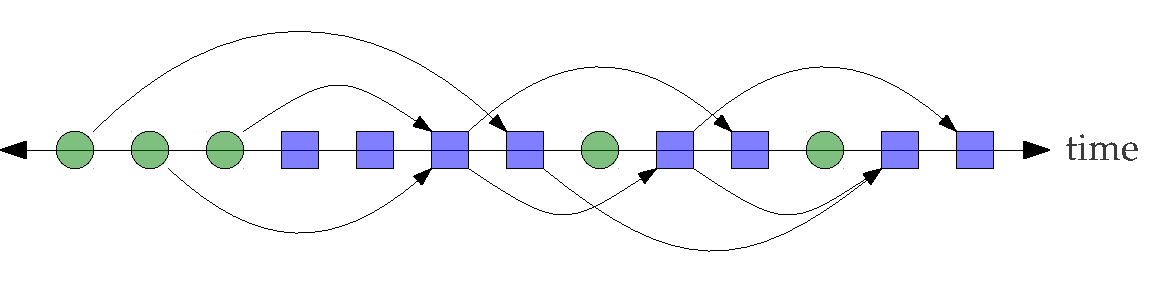
\includegraphics[width=10cm]{gfx/dependency_traces}
%\caption{Dependency traces as propagator cells.}
%\label{figure:propogators_dependency_traces}
%\end{figure}
